\section{Architecture}

\begin{figure}[t]
    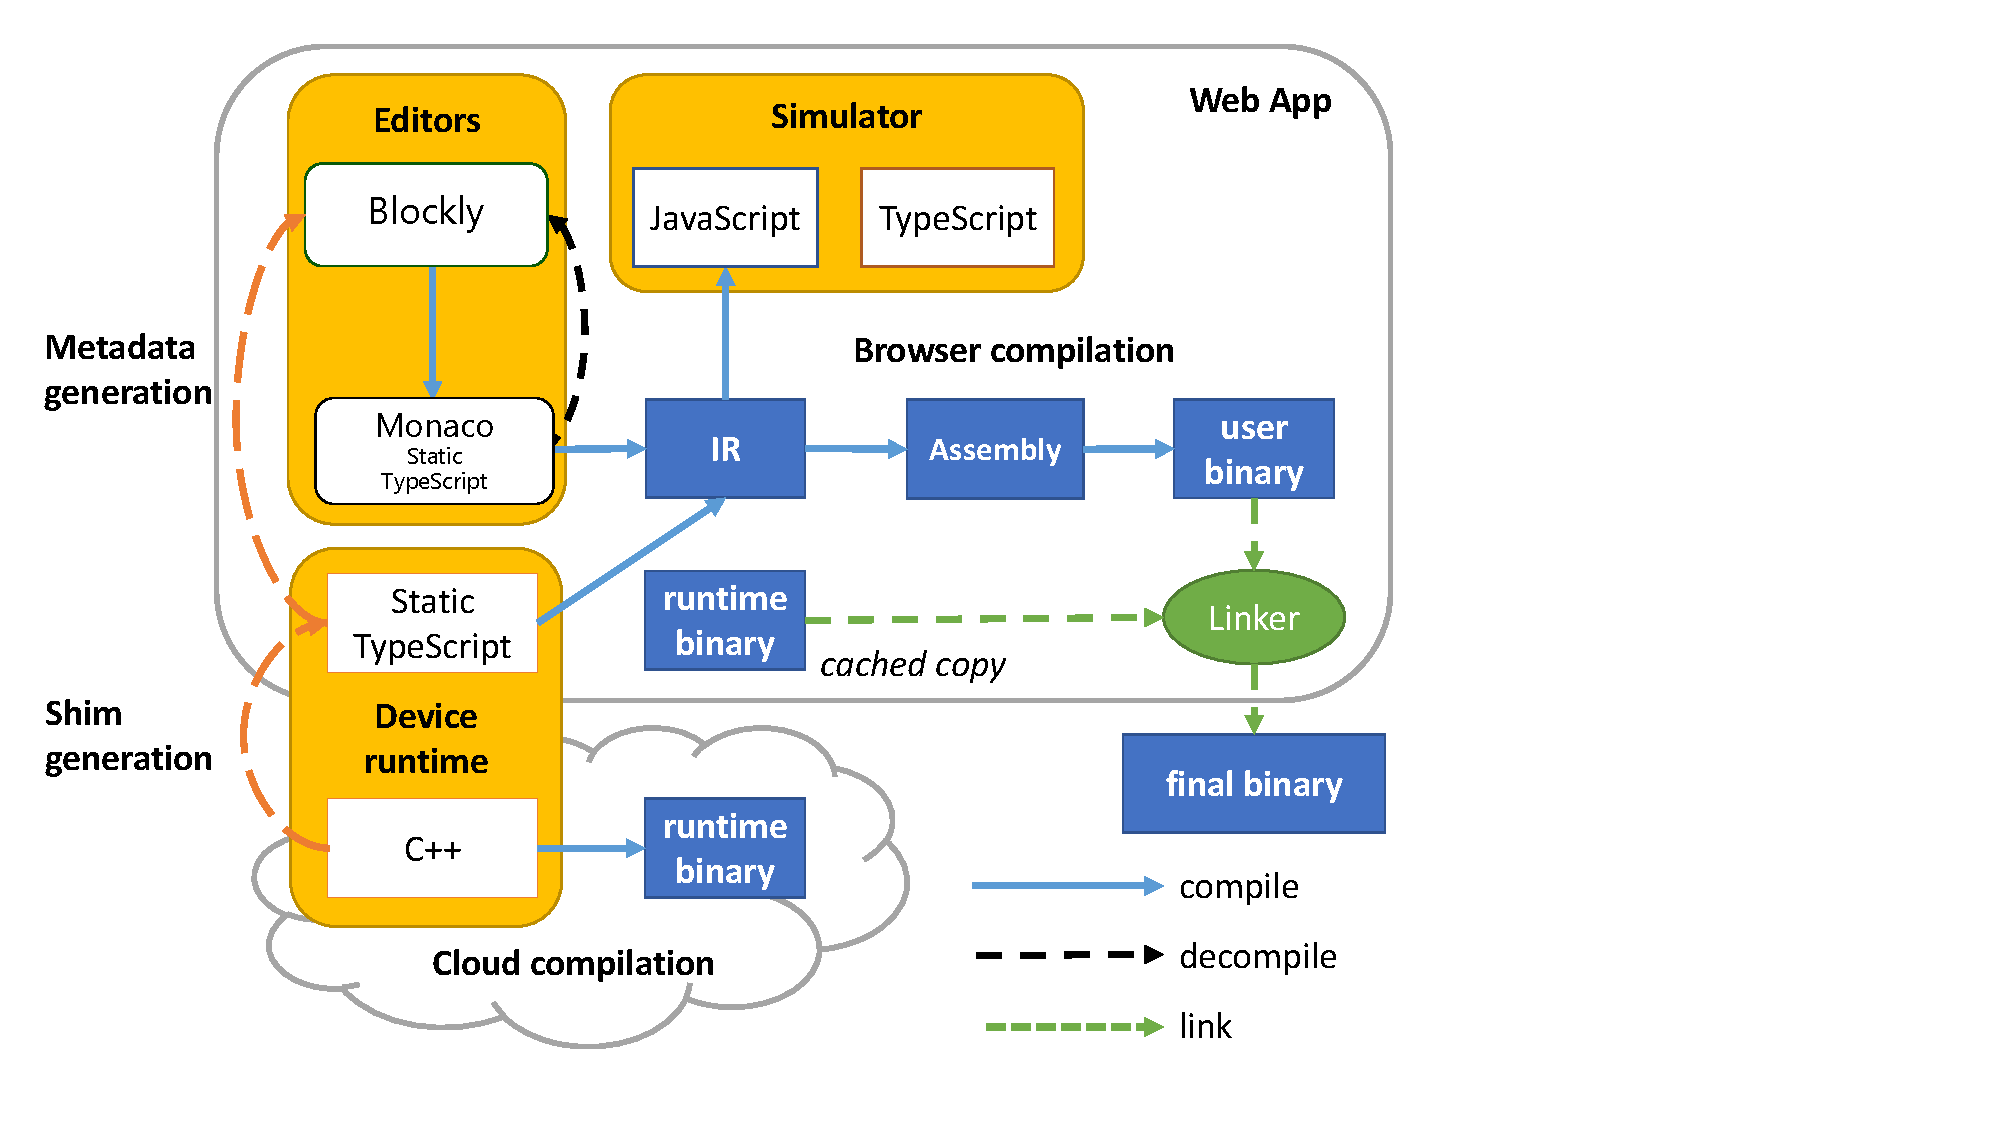
\includegraphics[width=4.8in]{makecodeFig.pdf}
\caption{\label{fig:makecode}\MC web app}
\end{figure}

The primary entry point to our platform, \MCN, is web-based, requires no installation, and supports the simplified asynchronous programming of MCUs via editors for visual blocks and textual JavaScript languages (Section~\ref{sec:makecode}). Supporting higher level languages is \CON a, component-oriented, event-driven, fiber-based C++ runtime environment that bridges the semantic gap between higher-level languages (such as TypeScript) and the hardware, modelling each hardware component as a software component. Enabling the programming of the microcontroller is \UFN, a new file format for simplified transfer of serial data (such as programs) to the device, using a driverless USB mass storage abstraction (Section~\ref{sec:uf2})

\MC can be accessed from any modern web browser and cached locally for \emph{entirely offline use}. The \MC web app incorporates the open source Blockly (\emph{\href{https://github.com/google/blockly}{blockly}}) and Monaco (\emph{\href{https://github.com/Microsoft/monaco-editor}{monaco-editor}}) editors (upper-left), an in-browser device simulator (upper-right) for testing programs before transferring them to the physical device, as well as \emph{in-browser compilation} of Static TypeScript to machine code and linking against the C++ runtime (\emph{\CON}), pre-compiled (by a cloud service, lower left)..

\MC devices appear as USB pen drives when plugged into a computer. After a user has finished developing a program, the compiled binary is ``downloaded'' locally to the users computer and then transferred (flashed) to the MCU (exposed as USB pen drive) by a simple file copy operation. No additional installation is required to program the MCU as drivers for pen drive come pre-installed on many operating systems (MacOS, Windows, Linux, Android, ChromeOS).

These advances enable beginners to get started programming MCUs from any modern web browser, and offer a safe environment for hardware vendors to innovate and add new components using Static TypeScript. All of the platform's components are open source on GitHub (links removed).